%           %experimenting with svn-multi

\svnkwsave{$RepoFile: siminos/froehlich/flow.tex $}
\svnidlong {$HeadURL$}
{$LastChangedDate$}
{$LastChangedRevision$} {$LastChangedBy$}
\svnid{$Id$}


\chapter{\CLf}
\label{chap:blog}

     \Private{
\noindent{\bf Rebecca -
Jun 16 - Aug 21 2009}:\\
     }
This project first reproduces results reported by
Siminos\rf{SiminosThesis}, and then investigates various ways
of `quotienting' the \SOn{2} symmetry of \cLe, and reducing
the dynamics to symmetry 4-dimensional \reducedsp.
     \PC{
   When you write
   a project report or a research article, you always write abstract, introduction
   and conclusions first, and then keep rewriting them often.
   They are the most important parts of the text, as that is
   for most people only parts they will look at.
   }


The project consists of my notes and exercises. The flow of
the argument is in the classical
\HREF{http://en.wikipedia.org/wiki/Socratic_method}{Socratic dialogue}
mode; question, answer, question, $\cdots$.
    %
    \Private{ % subversion label pages
$\footnotemark\footnotetext{{\tt \svnkw{RepoFile}}, rev. \svnfilerev:
 last edit by \svnFullAuthor{\svnfileauthor},
 \svnfilemonth/\svnfileday/\svnfileyear}$
    } % end \Private{

The \cLe\ were introduced by Gibbon and McGuinness\rf{GibMcCLE82}
as a low-dimensional model of baroclinic instability in the
atmosphere. In the complex form, they are given by
\beq
\begin{split}
 \dot{x} &=-\sigma x+ \sigma y \\
 \dot{y} &=(r-z)x-a y \\
 \dot{z} &= \frac{1}{2}\left(x y^*+x^*y\right)-b z\,
 \label{eq:CLe}
\end{split}
\eeq
where $x,y$, $r=r_1+ i\,r_2$, $a=1+i\,e$ are complex and $z$,
$b$, $\sigma$ are real. Rewritten in terms of real variables
$x=x_1+ i\, x_2\,,\ y=y_1+i\, y_2$, \cLe\ are a 5-dimensional
first order ODE system\rf{SiminosThesis}
\beq
\begin{split}
	\dot{x}_1 &= -\sigma x_1 + \sigma y_1\\
	\dot{x}_2 &= -\sigma x_2 + \sigma y_2\\
	\dot{y}_1 &= (r_1-z) x_1 - r_2 x_2 -y_1-e y_2 \\
	\dot{y}_2 &= r_2 x_1 + (r_1-z) x_2 + e y_1- y_2\\
	\dot{z} &= -b z + x_1 y_1 + x_2 y_2\,.
	\label{eq:CLeR}
\end{split}
\eeq
In all numerical calculations that follow we shall set the
parameters to the Siminos values\rf{SiminosThesis},
\beq
r_1=28,\; b=\frac{8}{3},\;
\sigma=10,\; e=\frac{1}{10},\quad \mbox{and} \quad r_2=0
\,.
\ee{SiminosPrmts}

Here we are not interested in the physical applications of
these equations; rather, we study them as a simple example of
a dynamical system with continuous (but no discrete)
symmetries. Our goal is to find computationally
straightforward method of reducing the dynamics to a
lower-dimensional \statesp, where each group orbit of the
full system (\ie, set of translationally equivalent states)
is represented by a single point. If successful, the methods
that we develop might be applicable to very high-dimensional
flows, such as translationally equivariant fluid flows
bounded by pipes or planes\rf{GHCW07,GibsonMovies}.

\noindent {\bf Acknowledgments.}
S.F. work was supported by the National Science Foundation
grant DMR~0820054.
P.C. thanks Glen Robinson Jr. for support.

\subsection{Visualizing \cLf}

In \refexer{exer:PlotCLf} we simulate \cLf\ in order to
visualize its long-time dynamics, as in
\reffig{fig:CLEx1x2z}. The dynamics is a big mess - the
trajectory seems to oscillate while drifting around $z$-axis.
Of most importance in \reffig{fig:CLEx1x2z}, is to notice
that the flow has a rotational symmetry about the $z$-axis.
Throughout the rest of the project we will try to find more
illuminating ways of understanding the dynamics of this flow
as well as ways of "cleaning it up"--that is, removing this
symmetry and reducing the ODE system from five dimensions to
four.
%    \PC{label axes, use legible fonts in all figures.}
%    \PC{put all single figures into SFIG format, as
%        \reffig{fig:CLEx1x2z}.}
                                                    \exerbox{exer:PlotCLf}

%%%%%%%%%%%%%%%%%%%%%%%%%%%%%%%%%%%%%%%%%%%%%%%%%%
% computed by graphs.nb
\SFIG{CLEx1x2z}
{}{
A typical $\{x_1,x_2,z\}$ plot of the \cLf\ strange attractor,
with initial point
$(x_1, x_2, y_1, y_2, z) = (1, 0, 0, 1, 1)$.
    }{fig:CLEx1x2z}
%%%%%%%%%%%%%%%%%%%%%%%%%%%%%%%%%%%%%%%%%%%%%%%%%%


\section{Linear stability}
\label{sect:stability}
%\PC{Write up here the general text on stability, following \refref{DasBuch},
%\\
%\wwwcb{/chapters/stability.pdf}
%    }
In our first attempt to understand the dynamics of the flow, we examine its stability by finding the stability matrix $\Mvar$. This is the matrix of partial derivatives of $v(x)$,
\beq
\Mvar = \frac{\pde v}{\pde x}=
\left(\barr{ccccc}\medskip
\frac{\pde\dot{x}_1}{\pde x_1} & \frac{\pde\dot{x}_1}{\pde x_2} &\frac{\pde\dot{x}_1}{\pde y_1} & \frac{\pde\dot{x}_1}{\pde y_2} & \frac{\pde\dot{x}_1}{\pde z}\\\medskip
\frac{\pde\dot{x}_2}{\pde x_1} & \frac{\pde\dot{x}_2}{\pde x_2} &\frac{\pde\dot{x}_2}{\pde y_1} & \frac{\pde\dot{x}_2}{\pde y_2} & \frac{\pde\dot{x}_2}{\pde z}\\\medskip
\frac{\pde\dot{y}_1}{\pde x_1} & \frac{\pde\dot{y}_1}{\pde x_2} &\frac{\pde\dot{y}_1}{\pde y_1} & \frac{\pde\dot{y}_1}{\pde y_2} & \frac{\pde\dot{y}_1}{\pde z}\\\medskip
\frac{\pde\dot{y}_2}{\pde x_1} & \frac{\pde\dot{y}_2}{\pde x_2} &\frac{\pde\dot{y}_2}{\pde y_1} & \frac{\pde\dot{y}_2}{\pde y_2} & \frac{\pde\dot{y}_2}{\pde z}\\
\frac{\pde\dot{z}}{\pde x_1} & \frac{\pde\dot{z}}{\pde x_2} &\frac{\pde\dot{z}}{\pde y_1} & \frac{\pde\dot{z}}{\pde y_2} & \frac{\pde\dot{z}}{\pde z}\\
\earr\right)
\label{5x5stabMat}
\eeq
For the \cLe\ it is the $[5\!\times\!5]$ matrix,
                                                    \exerbox{exer:StabmatCLf}
\beq
  \Mvar =\left(\barr{ccccc}
    -\sigma    	& 0 		& \sigma & 0    &  0 \\
	0 	& -\sigma       & 0      & \sigma   &  0 \\
	r_1-z  &     -r_2      & -1     & -e & -x_1 \\
	r_2     & r_1-z       	& e  	& -1       & -x_2 \\
	y_1     & y_2           & x_1    & x_2      & -b
    \earr\right)
\eeq
As explained in ChaosBook.org\rf{DasBuch}, a stability matrix
describes the instantaneous rate of shearing of the
infinitesimal neighborhood of $x(t)$ by the flow. That is, it
describes how quickly points initially very near to $x(t)$ will
diverge away from it in time. It is the matrix of
velocity gradients. This matrix $\Mvar$ is also an important
tool which we will use later on.


\section{\Eqva}

An \eqv\ $\EQV{}$ is a point $\ssp_{\EQV{}}$ for which the
velocity field of an ordinary differential equation
$\dot{\ssp} = v(\ssp)$ is zero, $v(\ssp_{\EQV{}})=0$. These
are points where the flow does not move, and if it reaches an
equilibrium, the flow remains there. For the \cLe\, the only
equilibrium we found was at the origin $\EQV{0}=(0, 0, 0, 0,
0)$. If we could set this {\em infinitely precisely} as the
initial point of the flow, instead of seeing the messiness of
\reffig{fig:CLEx1x2z}, we would stay at this single point for
all times. In any simulation, the (finite precision)
trajectory eventually leaves this point.
                                                    \exerbox{exer:EquiCLe}

\subsection{Stability of \eqva}
At an equilibrium, the flow manages to stay at a single
point, but what if we start at points near the equilibrium? Will
they collapse into the equilibrium, or will they diverge away
from it? In order to answer this, we find and examine the
eigenvalues and eigenvectors of \Mvar\ evaluated at the
equilibrium $\EQV{0}$.
                                                    \exerbox{exer:EigenE0}
For the \cLe\, we find that the eigenvalues are
        \PC{ChaosBook convention is to order eigenvalues
        from most positive (unstable) to the most negative,
        that is why I renumbered them. Try to follow that
        everywhere. Replace complex eigenvectors by the real,
        imaginary parts, as that is what you actually use - I
        did this in \refeq{eigVecQ1}. I might have introduced
        errors in renumbering them, so trust your own
        computations, especially regarding the
        \reffig{fig:CLEE0} comments.
        }
\beq
\begin{split}
\lambda_{1,2} &=11.8277 \pm 0.062985 i\\
\lambda_{3,4} &=-22.8277 \pm 0.037015 i\\
\lambda_5 &=-2.66667\\
\end{split}
\eeq
with the associated eigenvectors
    \PC{\label{suspectEigVecs}is suspect:
    real, im parts seem interchanged in $e_1$?}
\bea
e_{1} &=& e_2^* =(0.001321+0.4581 i, 0.4581-0.001321 i, i, 1, 0)
\label{suspectEigVecs}\\
e_3 &=& e_4^* = (0.002249-0.7795 i, -0.7795-0.002249 i, 2.8421+i, 1, 0)
\continue
e_5 &=& (0, 0, 0, 0, 1)
\,.
\nnu
\eea
By examining the eigensystem, we can get a sense of what
happens to points near the equilibrium $\EQV{0}$. The
numerical values of the real parts of the eigenvalues
determine how quickly the flow will converge onto or diverge
away from the equilibrium. For a positive real part the flow
will diverge, and for a negative real part it will converge.
Complex eigenvalues also indicate that the motion will be
spiraling.

For the \cLe\ equilibrium $\EQV{0}$, the values of the
imaginary parts are orders of magnitude smaller than the real
parts, so that there will be very little spiraling. The large
values of the real parts tell us that the flow will
diverge/converge from the equilibrium very quickly.
                                                    \exerbox{exer:PlotEigenE0}

To illustrate this, we plot the eigenvectors (as real and
imaginary parts) and the flow at initial points very close to
$\EQV{0}$. The two real vectors (corresponding to a single
complex eigenvector) define the plane in which the flow will
spiral. We initiate the flow very close to $\EQV{0}$ at a
point along one of these vectors. In \reffig{fig:CLEE0},
    \RW{
    I'm still having trouble with this figure and
    matching up it's eigenvalues. In the Mathematica notebook
    where it was computed (eigensystem.nb), the "yellow"
    eigenvectors that are plotted are labeled $e3$, which
    numerically matches the second vector in the list of computed
    eigenvectors (at the time, we called the all-real vector
    $e1$). The second eigenVALUE which would correspond to this
    yellow-$e3$ vector is -22... Predrag says it should be the
    +11...eigenvalue, but I can't find how they match up
    correctly. I have double and triple-checked all of the
    subscripts and as far as I can tell, the vectors in the plot
    are $e_4$, as listed here in this paper (not the $e4$ in
    Mathematica) and have eigenvalue -22. Will continue on
    ignoring this problem, I'm hoping I just missed something.
    }
we can see that for the vectors with a very small imaginary
part and a positive real part, the flow does not spiral
noticeably and that it diverges away from the equilibrium very
quickly.
%%%%%%%%%%%%%%%%%%%%%%%%%%%%%%%%%%%%%%%%%%%%%
% computed by eigensystem.nb
\SFIG{ProblemsPill} %CLEE0}
{}{
$\{x_1, x_2, z\}$ plot of the expanding eigenvector $e_1$
(red) and the contracting eigenvector $e_4$ (yellow) of the
\eqv\ $E_0$ \stabmat\ of \cLf, with initial point at $\frac{1}{100}
e_4$.
}
{fig:CLEE0}
%%%%%%%%%%%%%%%%%%%%%%%%%%%%%%%%%%%%%%%%%%%%%


\section{Symmetries of dynamics}
\label{sect:SymmDyn}

         \Private{
\noindent{\bf Rebecca -
Jun 18 2009}:\\
\medskip\noindent
         }
In order to eventually remove the rotational symmetry in the
\cLf\, we need to show that the flow is rotationally
equivariant. By showing this, we will then be able to apply
algorithms to remove the symmetry. Rotational equivariance in
this situation will let us commute a rotation operator with
taking time derivatives.\RW{I plan on writing more here, just
haven't thought of what else I want to say yet.}

We begin by defining `equivariance.'
A flow $\dot{x}= v(x)$ is equivariant under an operation $\mathbb{G}$ when
\beq
\mathbb{G} \cdot v(x)=v(\mathbb{G} \cdot x)
\,.
\ee{eq:FiniteRot}
An element of a compact Lie group that is continuously connected to the identity can be expressed as
\beq
\mathbb{G}(\theta)=e^{{\theta} \Lg }\,,\theta \Lg = \sum \theta_a \Lg_a
\ee{FiniteRot}
where the $\Lg_a$ are the generators of infinitesimal transformations and the $\theta_a$ are the parameters.
                                                    \exerbox{exer:FinRot2d}
For an infinitesimal rotation, $\theta \ll 1$,
\[
\mathbb{G}(\theta)=1+\theta  \Lg  + \cdots
\,,
\]
the statement of equivariance
$
\dot{x}=\mathbb{G}^{(-1)} \cdot v(\mathbb{G} \cdot x)
$
becomes
\[
\dot{x}=(1-\theta \Lg ) \cdot v(x+\theta  \Lg \cdot x) + \cdots
       =v(x)-\theta \left(
            \Lg \cdot v(x) - \frac{dv}{dx} \cdot \Lg \cdot x
                     \right)  + \cdots
\,.
\]
The $\dot{x}$ and $v(x)$ cancel, and the $\theta$ can be
divided out. We are left with the {\em infinitesimal
rotations} version of the equivariance condition
\refeq{eq:FiniteRot}:
\beq
0=- \Lg \cdot v(x)+\Mvar \cdot \Lg \cdot x
\,,
\label{eq:InfnmslRot}
\eeq
where $\Mvar = \frac{\pde v}{\pde x}$ is the \stabmat\ \refeq{5x5stabMat}.

We have used both this infinitesimal rotation condition and
the finite angle rotation condition \refeq{eq:FiniteRot}, to
verify that the \cLe\ are rotationally equivariant.
                                                    \exerbox{exer:InfinRotInvari}
                                                    \exerbox{exer:FinRotInvarCmplx}
                                                    \exerbox{exer:FinRotInvari}


\section{\Reqva}

To further visualize the drifting of the flow around the
$z$-axis, we next find and plot the relative equilibria of
the \cLe. A relative equilibrium is a solution of the flow
which appears stationary in a frame rotating at the
appropriately chosen constant angular velocity. We find these
points in a manner similar to finding the equilibria, with
one difference. As the flow drifts (rotates), a relative
equilibrium will drift as well, so that instead of setting
all of the $v(x)=0$, we allow the component of $v(x)$ tangent
to direction of group rotation to be non-zero. This tangent is not
necessarily easily defined in the
Cartesian coordinates which we have so far been using. The
relative equilibrium is more conveniently determined  in
polar coordinates.

\subsection{Equations in the polar form}
\label{sect:coordChange}
\PC{Gilmore and Letellier\rf{GL-Gil07b} is a good reference
        for a discussion of such coordinate changes}
We can rewrite the \cLe\ to polar coordinates using the definition
\beq
(x_1,x_2,y_1,y_2,z) =
    (\rho_1 \cos\theta_1,\rho_1\sin\theta_1,
     \rho_2\cos\theta_2,\rho_2\sin\theta_2,z)
\,,
\label{eq:CartToPol}
\eeq
and come up with the new equations
\[ %\beq
\left(
\begin{array}{c}
\dot{\rho}_1\\
\dot{\theta}_1\\
\dot{\rho}_2\\
\dot{\theta}_2\\
\dot{z}
\end{array}
\right)
=
\left(
\begin{array}{c}
 -\sigma\left(\rho_1 - \rho_2\cos\theta\right) \\
 -\sigma\frac{\rho_2}{\rho_1}\sin \theta  \\
 -\rho_2 + \rho_1\left((r_1-z)\cos \theta - r_2 \sin\theta\right)\\
  e  + \frac{\rho_1}{\rho_2}\left((r_1-z)\sin\theta +r_2 \cos\theta\right)\\
 -b z + \rho_1\rho_2\cos\theta
\end{array}
\right)
,
\] %\ee{eq:PolarCLe}
                                                    \exerbox{exer:HarmOscPolar}
                                                    \exerbox{exer:polarCLe}
We know from classical mechanics that for translationally or
rotationally invariant flows the relative distance is
invariant (that is why one speaks of `relative' equilibria),
hence we introduce a variable $\theta = \theta_1-\theta_2$.
This is the variable which allows us to
ultimately find the relative equilibria. As the flow is
rotating, $\theta_1$ and $\theta_2$ are changing, but, at the
relative equilibria, the difference between them is constant.
This new variable also allows us to rewrite the \cLe\ yet
again, this time in only four dimensions.
\beq
\left(
\begin{array}{c}
\dot{\rho}_1\\
\dot{\rho}_2\\
\dot{\theta}\\
\dot{z}
\end{array}
\right)
=
\left(
\begin{array}{c}
 -\sigma\left(\rho_1 - \rho_2\cos\theta\right) \\
 -\rho_2 + (r_1-z)\rho_1\cos \theta\\
  -e -\left(\sigma\frac{\rho_2}{\rho_1}
 +(r_1-z)\frac{\rho_1}{\rho_2}\right)\sin\theta\\
 -b z + \rho_1\rho_2\cos\theta
\end{array}
\right)
\label{eq:PolarCLeTheta}
\eeq

%%%%%%%%%%%%%%%%%%%%%%%%%%%%%%%%%%%%%%%%%%%%%%%%%%
% computed by PCsimul.nb
\SFIG{ProblemsPill} %PCsimulPolar}
{}{
A polar coordinates $\{\rho_1,\rho_2,\theta\}$ plot of the
\cLf\ strange attractor. $\theta$ is very small until the
trajectory approaches either $\rho_1 \to 0$ or $\rho_2 \to
0$, where \texttt{Mathematica} continues through the
singularity by a rapid change of $\theta$ by $\pi$.
$\rho_1 = \rho_2 =
0$ separates the two folds of the attractor.
    }{fig:PCsimulPolar}
%%%%%%%%%%%%%%%%%%%%%%%%%%%%%%%%%%%%%%%%%%%%%%%%%%
                                                    \exerbox{exer:PlotPolarCLf}
Plotting these equations, we see that the polar
representation introduces singularities into what initially
was a smooth flow, as shown in \reffig{fig:PCsimulPolar}. We
shall encounter the same problem in implementing the $x_1=0$
moving frames \slice, see \reffig{fig:PCunrot1}.

\subsection{Computing and plotting the relative equilibrium $\REQB{1}$}

To compute the relative equilibria, we use a method similar to finding the equilibria. We set $(\dot\rho_1, \dot\rho_2, \dot\theta, \dot z)=(0, 0, 0, 0)$ and solve the set of equations numerically. We find that there are 8 solutions to the system, all differing by only positive and negative signs and variations of
\beq
(\rho_1,\rho_2,\theta,z) =
\left(\sqrt{b \,(r_1-d)},\sqrt{b d \,({r_1}-d}),
      \pm \cos^{-1}\left({1}/{\sqrt{d}}\right),
      r_1-d\right)
\label{eq:E1-PC}
\eeq
where $d=1 + {e^2}/{(\sigma +1)^2}$.
                                                    \exerbox{exer:CompRelEqu}

\refFig{fig:CLEPolEqui} shows a plot of the \cLf\ in polar
coordinates with initial point at the relative equilibrium,
$\REQB{1}$. As for an equilibrium, the flow should stay at a
single point (in these polar coordinates), however, numerical
errors eventually accumulate and the flow leaves $\REQB{1}$.
   \RW{is this true? {\bf PC:} yes. Also, your
   initial finite error is not in the spiral-out
   plane, hence the initial transient.}
                                                    \exerbox{exer:PlotPolEqu}
%%%%%%%%%%%%%%%%%%%%%%%%%%%%%%%%%%%%%%%%%%%%
% computed by equilibrium.nb
\SFIG{ProblemsPill} %CLEPolEqui}
{}{
$\{\rho_1,\rho_2,z\}$ plot of the \cLf, with initial point
at $\REQB{1}$.
}
{fig:CLEPolEqui}
%%%%%%%%%%%%%%%%%%%%%%%%%%%%%%%%%%%%%%%%%%%%

We can compute $\REQB{1}$ in Cartesian coordinates by fixing
the value of $\theta_1$ or $\theta_2$ and using the
definitions in \refeq{eq:CartToPol}. We get
                                                    \exerbox{exer:PlotRelEqu}
\[\ssp_{\REQB{}1} = (8.48492,0.0771356,8.48562,0,26.9999)
\,.
\]
\refFig{fig:CLERelEqui} shows the \cLf\ with initial point at $\ssp_{\REQB{}1}$. The relative equilibrium begins by tracing out a circle around the $z$-axis, showing how the flow drifts. Eventually numerical errors accumulate and the circle turns into a "horn" shape when the flow begins to spiral out.
%%%%%%%%%%%%%%%%%%%%%%%%%%%%%%%%%%%%%%%%%%%%%%%%%%%%%%%
% computed in equilibrium.nb
\begin{figure}[h]
\begin{center}
(a) % ~\includegraphics[width=0.35\textwidth]{CLERelEqui}
(b) % ~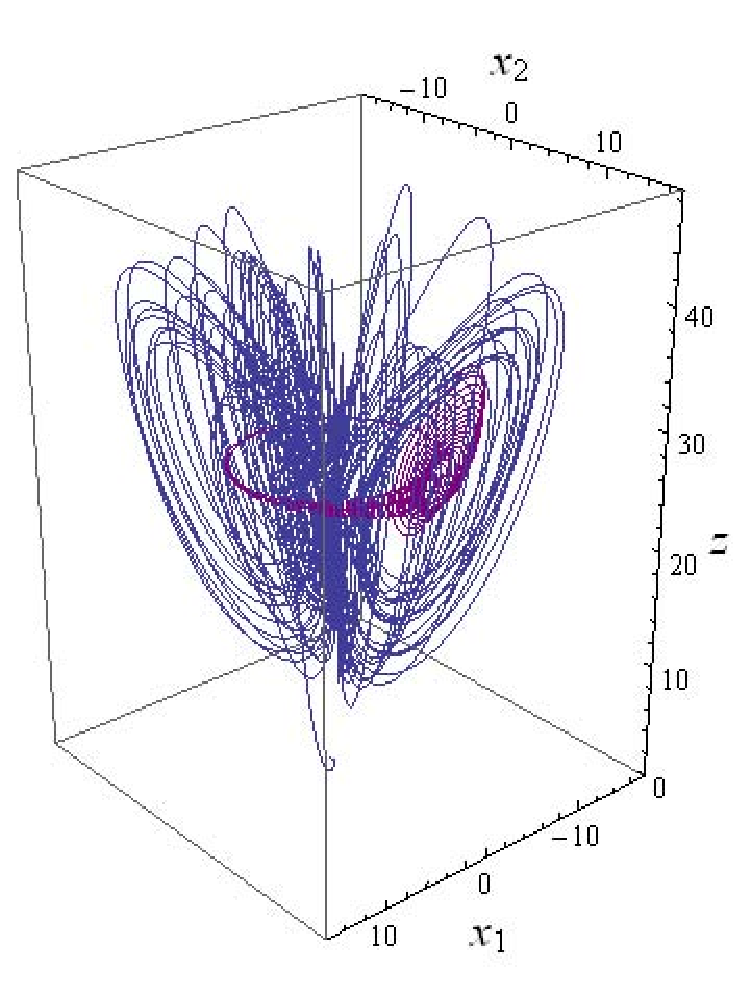
\includegraphics[width=0.35\textwidth]{CLEx1x2zRelEqu}
\end{center}
\caption{
Cartesian $\{x_1,x_2,z\}$ plot of the \cLf\ (a) with initial point
close to $\REQB{1}$, (b) superimposed over the strange attractor of
\reffig{fig:CLEx1x2z}.
    }
\label{fig:CLERelEqui}
\end{figure}
%%%%%%%%%%%%%%%%%%%%%%%%%%%%%%%%%%%%%%%%%%%%%%%%%%%%%%%

As discussed above, there are in total eight relative
equilibria. \refFig{fig:FourRelEquil} shows the flow with
initial point at four of these eight points and plotted in
Cartesian coordinates. Each of the initial points lies on the
circle. As the flow itself is rotationally invariant, all
of these eight relative equilibria are equivalent. From
here on, we only examine the properties of the point defined
above as $\ssp_{\REQB{}1}$.

%%%%%%%%%%%%%%%%%%%%%%%%%%%%%%%%%%%%%%%%%%%%
% computed by equilibrium.nb
\SFIG{ProblemsPill} %FourRelEquil}
{}{
Plot of four different relative equilibrium solutions (red,
yellow, green, blue). Some of the plots almost exactly
overlap and are not easily distinguishable.
}
{fig:FourRelEquil}
%%%%%%%%%%%%%%%%%%%%%%%%%%%%%%%%%%%%%%%%%%%%

\subsection{Eigen-system of the polar \stabmat}
As in \refsect{sect:stability}, we now find and plot the eigensystem of the stability matrix in order to understand the stability of $\REQB{1}$. Using the same methods described there, we find the eigenvalues
\[
(\lambda_{1,2},\lambda_3,\lambda_4)
= (0.0938179 \pm 10.1945 i,-11.0009,-13.8534)
\]
with the eigenvectors
\bea
\Re e_{1} &=& \Re e_{2} = (-0.266121, -0.0321133, 0.00034139, 0.719222)
\continue
\Im e_{1}  &=& -\Im e_{2} = (-0.295017, 0.569063, -0.000551886,0)
\continue
e_3 &=& (-0.0883591, -0.0851485, -0.989135, -0.0809553)
\continue
e_4 &=& (-0.855586, -0.329912, -0.00273531, -0.398902)
\,.
\label{eigVecQ1}
\eea

As in \refsect{sect:stability}, we can also plot the flow
(in polar coordinates) with an initial point very near to
$\REQB{1}$ along one of the eigenvectors.
\refFig{fig:CLEQ1} shows just this.
%%%%%%%%%%%%%%%%%%%%%%%%%%%%%%%%%%%%%%%%%%%%%%%%%%%%
% computed by eigensystem.nb
\begin{figure}[h]
\begin{center}
(a) %~\includegraphics[width=0.42\textwidth]{CLEQ1}
(b) %~\includegraphics[width=0.28\textwidth]{CLEQ1t100}
\end{center}
\caption{
(a) $\{\rho_1, \rho_2, z\}$ plot of the eigenvector $e_3$
(black) and the polar \cLf\ at initial values of
$\frac{1}{100}, \frac{2}{100}, \frac{3}{100}, \frac{4}{100},
\frac{5}{100},$ and $ \frac{6}{100}$ of $e_3$ (red, orange,
yellow, green, blue, violet) with $t$ from 0 to
$2\,\period{spiral}=1.232\cdots$, (b)
with initial point at $ \frac{6}{100} e_3$ (violet) and with
$t$ from 0 to 100.
    }
\label{fig:CLEQ1}
\end{figure}
%%%%%%%%%%%%%%%%%%%%%%%%%%%%%%%%%%%%%%%%%%%%%%%%%%%%%
                                                    \exerbox{exer:EigenQ1}
                                                    \exerbox{exer:PlotPolEigenQ1}

\section{\Reducedsp}
\label{sect:reducedStateSp}

Finally, we move on to the goal of the project, reducing the
state-space of the \cLe\ to only four dimensions. We present
two different versions of the `method of moving frames.' The
method can introduce singularities of the type we have
encountered in the polar coordinate reformulation, as in
\reffig{fig:PCsimulPolar}. We encounter these in applying
`polar' version of the method, but not in the other, more
general version. We finish by reproducing Siminos
`integration on the \csection' which - inspite of lacking a
theoretical justification - projects the \cLf\ to a nice
Lorenz-type attractor.

This section of the report is written in collaboration with
E.~Siminos and P.~Cvitanovi\'c.

\subsection{Method of moving frames, finite time steps}
\label{sect:MovFrame}

     \Private{
\noindent{\bf Predrag -
July 19, Aug 12 2009}: %\\
    }

Siminos\rf{SiminosThesis} discusses symmetry reduction by the
method of {\em moving frames} of Cartan\rf{CartanMF}, in the
formulation of Fels and
Olver\rf{FelsOlver98,FelsOlver99,OlverInv}.
                                                \exerbox{exer:SO2cSect}
The moving frames method allows the determination of (in
general non-polynomial) invariants of the group action by a
simple and efficient algorithm that, as argued in
\rf{SiminosThesis}, works well in high-dimensional \statesp s.
    \PC{Vaggelis, add references here? {\bf ES}: mmm...
SiminosThesis?} \PC{Vaggelis, why ``(non-polynomial)''
invariants? length$^2$ is polynomial {\bf ES}: In general we
don't get invariant polynomials 	from the moving frame
method applied to high dimensional representations of compact
Lie groups. 	For CLe we get a polynomial invariant and two
invariants that are rational functions of polynomials.
     }

Split up the integration of the $\SOn{2}$-equivariant ODE into
a sequence of short time steps, each followed by a rotation
such that the next segment initial point is in the point
$\ssp^{*}$ {\slice}, a $(d\!-\!1)$-dimensional hyperplane
normal to the group rotation tangent $t^{*}$ at point
$\ssp^{*}$:
\beq
(\ssp- \ssp^{*}) \cdot t^{*}=0
    \,,\qquad
t^{*} = \Lg \cdot \ssp^{*}
\,.
\ee{PCsectQ}
For any $\hat{\ssp}$, $\ssp =
\mathbb{G}(\theta)\cdot\hat{\ssp}$ is defined to be the
rotation of $\hat{\ssp}$ that lies in the \slice. Such a
map from a point in space to the group action is called a
\emph{moving frame} in the formulation of Fels and
Olver\rf{FelsOlver98,FelsOlver99,OlverInv}. A generic point
$\ssp^{*}$ not on the $z$ axis should suffice to fix a good
\slice, for example a point on an \reqv\ group orbit,
$\ssp^{*} = \ssp_{\REQB{}1}$.
                                                    \exerbox{exer:PCsectionCLe}
As $\ssp^{*} \cdot t^{*}=0$ by the antisymmetry of
$\Lg$, \refeq{PCsectQ} reduces to the condition
\beq
0 = \ssp \cdot \Lg \cdot \ssp^{*}
  %= \mathbb{G}(\theta) \cdot \hat{\ssp}   \cdot \Lg \cdot \ssp^{*}
	=\hat{\ssp} \cdot \mathbb{G}(\theta)^T \cdot \Lg \cdot \ssp^{*}
\ee{PCsectQ1}
that determines $\theta$ for a given $\hat{\ssp}$. Each
circle intersects the section exactly twice,  so there are
two solutions, separated by $\pi$. We select the one
with a smaller clockwise rotation angle into the \slice.
The $z$-axis invariant subspace is always within the section,
so this is a nice, globally transverse \slice.

%%%%%%%%%%%%%%%%%%%%%%%%%%%%%%%%%%%%%%%%%%%%%%%%%%
% computed by PCunrot.nb
\SFIG{ProblemsPill} %PCunrot}
{}{
Method of moving frames, finite time steps version: a
trajectory started on the \slice, with $\ssp_1^{(0)}
=0$, evolves for a finite time to a \statesp\ point with a
non-zero $\hat{\ssp}_1^{(1)}$. The {\em entire} \statesp\ is then
rotated (the `frame is moved') so that the equivalent point
on the circle lies on the \slice, $\ssp_1^{(1)} =0$.
Thus after every finite time step followed by a rotation the
trajectory returns to the 4$\dmn$ $\ssp_1 =0$
\reducedsp.
}
{fig:PCunrot}
%%%%%%%%%%%%%%%%%%%%%%%%%%%%%%%%%%%%%%%%%%%%%%%%%%

\refFig{fig:PCunrot} illustrates the method of moving frames,
finite time version, for a \slice\ motivated by the polar
form of the \cLe\ of \refsect{sect:coordChange}. It is
defined, for example, by taking
$(x^{*}_1,x^{*}_2,y_1^{*},y_2^{*})=(0,1,0,0)$,
$x_1=0,\,x_2>0$. Start at $\ssp^{(0)}$ with $\ssp_1^{(0)}
=0$, evolve for a finite time to $\hat{\ssp}^{(1)}$. Compute
the polar angle $\theta_1$ of $\hat{\ssp}^{(1)}_1$ in the
$(\ssp_1,\ssp_2)$ plane, and rotate the {\em entire}
\statesp\ (hence `moving frame') clockwise by $\theta_1$,
$\ssp^{(1)} = \mathbb{G}(\theta_1) \cdot \hat{\ssp}^{(1)}$,
to satisfy the $\ssp_1=0$ \slice\ condition. Repeat. The
trajectory remains in the 4$\dmn$ $\ssp_1=0$
\reducedsp.
    \PC{complete \refFig{fig:PCunrot}
        - need to draw a longer segment of the initial trajectory,
        to make it clearer that the whole segment is rotated.
       }

\subsection{Method of moving frames, differential formulation}
\label{sect:MovFrameODE}


\begin{bartlett}
I made a wrong mistake.
\bauthor{Yogi Berra}
\end{bartlett}

     \Private{
\noindent{\bf Predrag, Vaggelis -
Aug 13 2009}: %\\
    }
%\noindent{\bf Vaggelis -
%August 12 2009}: %\\
%\refeq{EqMotionMovFramePC} is correct, there are problems with the derivation.
%PC Aug 13 2009: fixed the details as suggested

                                                    \exerbox{exer:CLEsmall-x1x2}
                                                    \exerbox{exer:csectionCLeODE}
                                                    \exerbox{exer:csectionPhase}
                                                    \exerbox{exer:SiminosSlice}
Infinitesimal time version of the moving frames symmetry
reduction is attained by taking small time steps in
\reffig{fig:PCunrot} and dropping the higher order terms, as
in \refsect{sect:SymmDyn}. For infinitesimal  $d\theta$ we
set $\sin d\theta \approx d\theta$, $\cos d\theta \approx
1$, $\mathbb{G}(d\theta) \approx {1}+ d\theta \, \Lg $, and
the condition \refeq{PCsectQ} for rotating an infinitesimal
time evolution step $dx = v\,dt$ back into the \slice\
\[
0 = (\ssp + dx) \cdot \mathbb{G}(d\theta)^T \cdot \Lg \cdot \ssp^{*}
  \approx (\ssp + dt\,v) \cdot (1+ d\theta\,\Lg)^T \cdot \Lg \cdot \ssp^{*}
  \approx dt\,v \cdot \Lg \cdot \ssp^{*} - d\theta\,\ssp \cdot \Lg \cdot \Lg \cdot \ssp^{*}
\]
%\ES{It is $\Lg^T=-\Lg$.}
yields
\beq
d\theta \approx \frac{v \cdot \Lg \cdot \ssp^{*}}
                     { \ssp \cdot \Lg \cdot \Lg \cdot \ssp^{*}} \,  dt
\,.
\ee{MFdtheta}

%%%%%%%%%%%%%%%%%%%%%%%%%%%%%%%%%%%%%%%%%%%%%%%%%%
% File: infMF.xfig
\SFIG{ProblemsPill} %infMF}
{}{
Method of moving frames, infinitesimal formulation.
}
{fig:infMF}
%%%%%%%%%%%%%%%%%%%%%%%%%%%%%%%%%%%%%%%%%%%%%%%%%%

Let $u(\ssp)$ be the vector field that generates the flow in
the \reducedsp. According to \reffig{fig:infMF}, in
the limit that $\mathbb{G}(d\theta) \approx 1+d\theta\,\Lg$ the
infinitesimal time step under $u$ is connected to the time
step under $v$ by
    \PC{in \reffig{fig:infMF}:\\
        * Change $R$ into $\mathbb{G}$. \\
        * Draw $z$ axis
        (would lie horizontal in the present version, so tilt the figure).\\
        * Indicate $d\theta$ by drawing from origin, spanned by arc $x, x+v dt$.\\
        * Include a segment of the group-orbit ellipse, so $t^{*}$ is
          clearly visualized as a tangent.\\
        * Add arrows to $v dt$, $u dt$.
        }
\[
 \ssp+u\,dt=  (1+d\theta\Lg)\cdot(\ssp+v dt)\,.
\]
Dropping second order terms, dividing through with $dt$
\[
 u = v+\frac{d\theta}{dt} \,\Lg\cdot\hat{x}
 \,,
\]
and substituting \refeq{MFdtheta} gives the \reducedsp\ equations:
\beq
\dot{\ssp} = v - \frac{(v \cdot \Lg \cdot \ssp^{*})}{(\ssp \cdot\ssp^{*})_4}
                 \, \Lg \cdot \ssp
\,,
\ee{EqMotionMovFramePC}
where we have used the fact that
$- \ssp \cdot \Lg\cdot\Lg \cdot \ssp^{*}
 = (\ssp \cdot \ssp^{*})_4 =
    x_1 x_1^{*}
   +x_2 x_2^{*}
   +y_1 y_1^{*}
   +y_2 y_2^{*}
$
is the dot-product restricted to the 4-dimensional
representation of $\SOn{2}$. By construction, the motion
stays in the $(d\!-\!1)$-dimensional \slice.
                                                        \exerbox{exer:csectionReduced}
    \PC{
A more elegant derivation is given in
\refrefs{rowley_reconstruction_2000,rowley_reduction_2003},
and will be incorporated in \refref{SiminosThesis} and a coming article on this
topic.
    }

A generic  $ \ssp^{*}$ can be brought to form $ \ssp^{*} =
(0,1,y_1^{*},y_2^{*})$ by a rotation and rescaling. Then $\Lg
\cdot \ssp^{*}  = (1,0,y_2^{*},-y_1^{*})$, and
\beq
\frac{(v \cdot \Lg \cdot \ssp^{*})}{(\ssp \cdot\ssp^{*})_4} =
\frac{v_1 + v_3 y^{*}_2 -v_4 y^{*}_1}
     {x_2 + y_1 y^{*}_1 + y_2 y^{*}_2}
%\frac{v_1 x^{*}_2 -v_2 x^{*}_1 + v_3 y^{*}_2 -v_4 y^{*}_1}
%     {v_1 x^{*}_1 + v_2 x^{*}_2 + v_3 y^{*}_1 + v_4 y^{*}_2}
\,.
\label{PCsectSin}
\eeq

%
%%%%%%%%%%%%%%%%%%%%%%%%%%%%%%%%%%%%%%%%%%%%%%%%%%%%%%%%%%%%%%%%%%
% CLEpcSect.png computed by  CLEfinal.nb (repo: vaggelis)
% CLEpcSect2.png computed by CLEfinal.nb (repo: vaggelis)
\begin{figure}[ht]
\begin{center}
(a) % 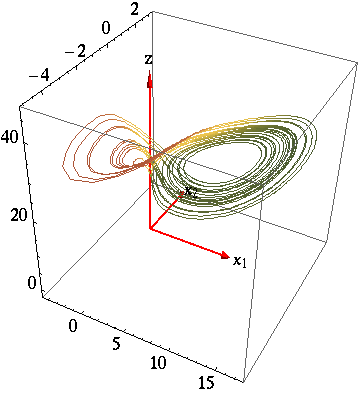
\includegraphics[width=0.40\textwidth]{CLEpcSect}
(b) %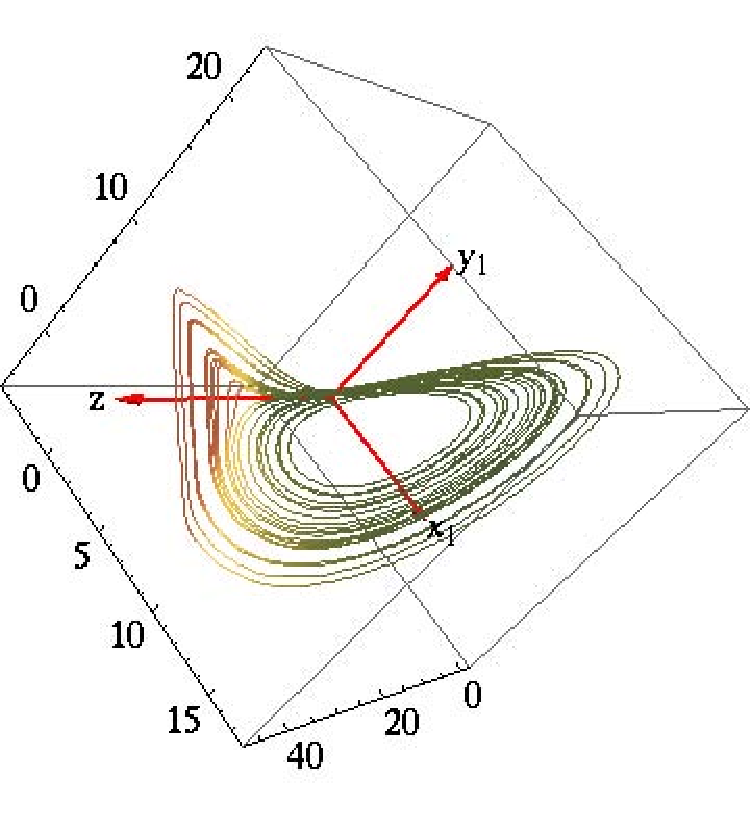
\includegraphics[width=0.43\textwidth]{CLEpcSect2}
\end{center}
\caption{
Method of moving frames, \slice\ fixed by a point on an
\reqv\ group orbit, $\ssp^{*} = \ssp_{\REQB{}1}$. The strange
attractor of \reffig{fig:CLEx1x2z} in the \reducedsp\
of \refeq{EqMotionMovFramePC}:
(a) $\{x_1,x_2,z\}$ projection,
(b) $\{x_1,y_1,z\}$ projection.
Color-coding indicates $(\hat{\ssp} \cdot \hat{\ssp^{*}})_4$
where $\hat{.}$ stands for unit vector, with green indicating values
of the inner product close to $1$ and brown indicating values
close to $0$.
    }
\label{fig:CLEpcSect}
\end{figure}
%%%%%%%%%%%%%%%%%%%%%%%%%%%%%%%%%%%%%%%%%%%%%%%%%%%%%%%%%%%%%%%%
%
A long time trajectory of \refeq{EqMotionMovFramePC} with
$x^*$ on the \reqv\ \REQB{1} group orbit is shown in
\reffig{fig:CLEpcSect}.
\ES{I will add a scale in \reffig{CLEpcSect} but it is too
late here to do it tonight.}
As initial condition
we chose an initial point on the unstable manifold
of \REQB{1}, rotated back to the \slice\ by angle $\theta$ as
prescribed by \refeq{PCsectQ1}. In \reffig{fig:CLEpcSect} we
show the part of the trajectory for $t\in\left[70,100\right]$.
The \reqv, now an equilibrium of the
\reducedsp\ dynamics, organizes the flow into a R\"ossler type
attractor. There appears to be no singularity in this
attractor although we can run into trouble with
\refeq{EqMotionMovFramePC} wherever the denominator in
\refeq{MFdtheta} vanishes, \ie, the direction of group
action on the point $\ssp$ is perpendicular to the direction
of group action on $\ssp^*$.
                                                        \exerbox{exer:PCsectionCLe}
    \PC{ in \reffig{fig:CLEpcSect}:\\
        * Mark $\ssp_{\REQB{}1}$ \\
        * Draw stable eigenvector of $\ssp_{\REQB{}1}$\\
        * State value of $\ssp_{\REQB{}1}$ somewhere
        }


%%%%%%%%%%%%%%%%%%%%%%%%%%%%%%%%%%%%%%%%%%%%%%%%%%
% computed by PCunrot.nb
\SFIG{ProblemsPill} %PCunrot1}
{}{
Method of moving frames, continuous time version, for the
polar coordinates motivated $x^{*}=(0,1,0,0)$,
$x_1=0,\;x_2>0$, \slice. The strange attractor of
\reffig{fig:CLEx1x2z} in the \reducedsp,
$\{x_2,y_2,z\}$ projection exhibits a discontinuity at
$x_2=0$.
}
{fig:PCunrot1}
%%%%%%%%%%%%%%%%%%%%%%%%%%%%%%%%%%%%%%%%%%%%%%%%%%

Indeed, the method appears to encounter singularities in
subsets of \statesp\rf{SiminosThesis}.
For example, the \reducedsp\ equations \refeq{PCsectSin}
for the polar coordinates inspired \slice\
$x^{*}=(0,1,0,0)$, $x_1=0,\;x_2>0$,
%this is illustrated by \reffig{fig:PCunrot}.
%$(\rho_1,\theta_1)$ are polar coordinates, $\rho_1 =
%\sqrt{\ssp_1^{ 2} + \ssp_2^{2}}$, see \refeq{eq:CartToPol},
are given by
                                                    \exerbox{exer:csectionCLe}
\beq
\dot{\ssp} = v - \frac{v_1}{\ssp_2} \Lg \cdot \ssp
\,.
\ee{EqMotionMovFrame}
A typical trajectory is shown in \reffig{fig:PCunrot1}.
The problem with defining the \slice\ by
\refeq{EqMotionMovFrame} is apparently that it fixes rotations
in the $(\ssp_1,\ssp_2)$ plane, not the full 4\dmn\ space.

\subsection{Integration on the \csection}

\RW{We never really talked too much about this, and I'm not
sure that I understand it all that well. This is mostly what
I figured out last night on my own. You may want to check it
for being...true. It was also very late when I wrote it, so
it may not be entirely comprehensible.
{\bf PC:} seems OK.}
Our second method of symmetry reduction Siminos
\rf{SiminosThesis} calls {\em integration on the
\csection\ (II)}. Here, we use the projection operator
\beq
\PperpOp_{ij}(\ssp^{*})=\delta_{ij}-
\frac{(\Lg \cdot \ssp^{*})_i (\Lg \cdot \ssp^{*})_j}{(\Lg \cdot \ssp^{*})^2}
\eeq
to remove any components of the \cLe\ that are tangent to the
rotation about the $z$-axis. Unlike the method of moving
frames where we continually rotate points back to the
{\slice}, in this method the components of integration are
tangent to the rotation only when crossing the hyperplane
fixed by $\ssp^{*}$. We define the new flow
$\frac{dx}{dt}=\PperpOp(x^{*}) v(x)$, following
Siminos\rf{SiminosThesis}, as
\beq
\dot x_{\perp} = v(x)-\mathbb{T}x^{*}
  \frac{\mathbb{T}x^{*}\cdot v(x)}{(\mathbb{T}x^{*})^{2}}
\label{eq:IntSlice}
\eeq\,
where $\Lg$ is the same as defined above and $x^{*}$ is an
arbitrary point defining the {\csection}.
\RW{I'm having a
problem understanding this equation, now that I look at it
closer, it doesn't quite match the method used in Mathematica
notebooks PCunrot.nb or my unrotate.nb. Unless I'm
misunderstanding something, the denominator doesn't quite
fit? Is this just a typo or am I very tired?
{\bf PC:} Tired. Never again write the report the last night of the
project, research cannot be crammed.}
This approach results in a nice 4-dimensional projection of
the \cLf,  as Siminos showed in
\reffig{fig:CLEtransvII}\,(a). Using \refeq{eq:IntSlice}, we
were able to reproduce this in \reffig{fig:CLEtransvII}\,(b).
However, as we were not able to establish a  theoretical
foundation for this projection, it remains only an
interesting visualization suggested by the method of moving
frames, not a viable method for symmetry reduction in its own
right.

%%%%%%%%%%%%%%%%%%%%%%%%%%%%%%%%%%%%%%%%%%%%%%%%%%%%%%%%%%%%%%%%%%
\begin{figure}[ht]
\begin{center}
(a) %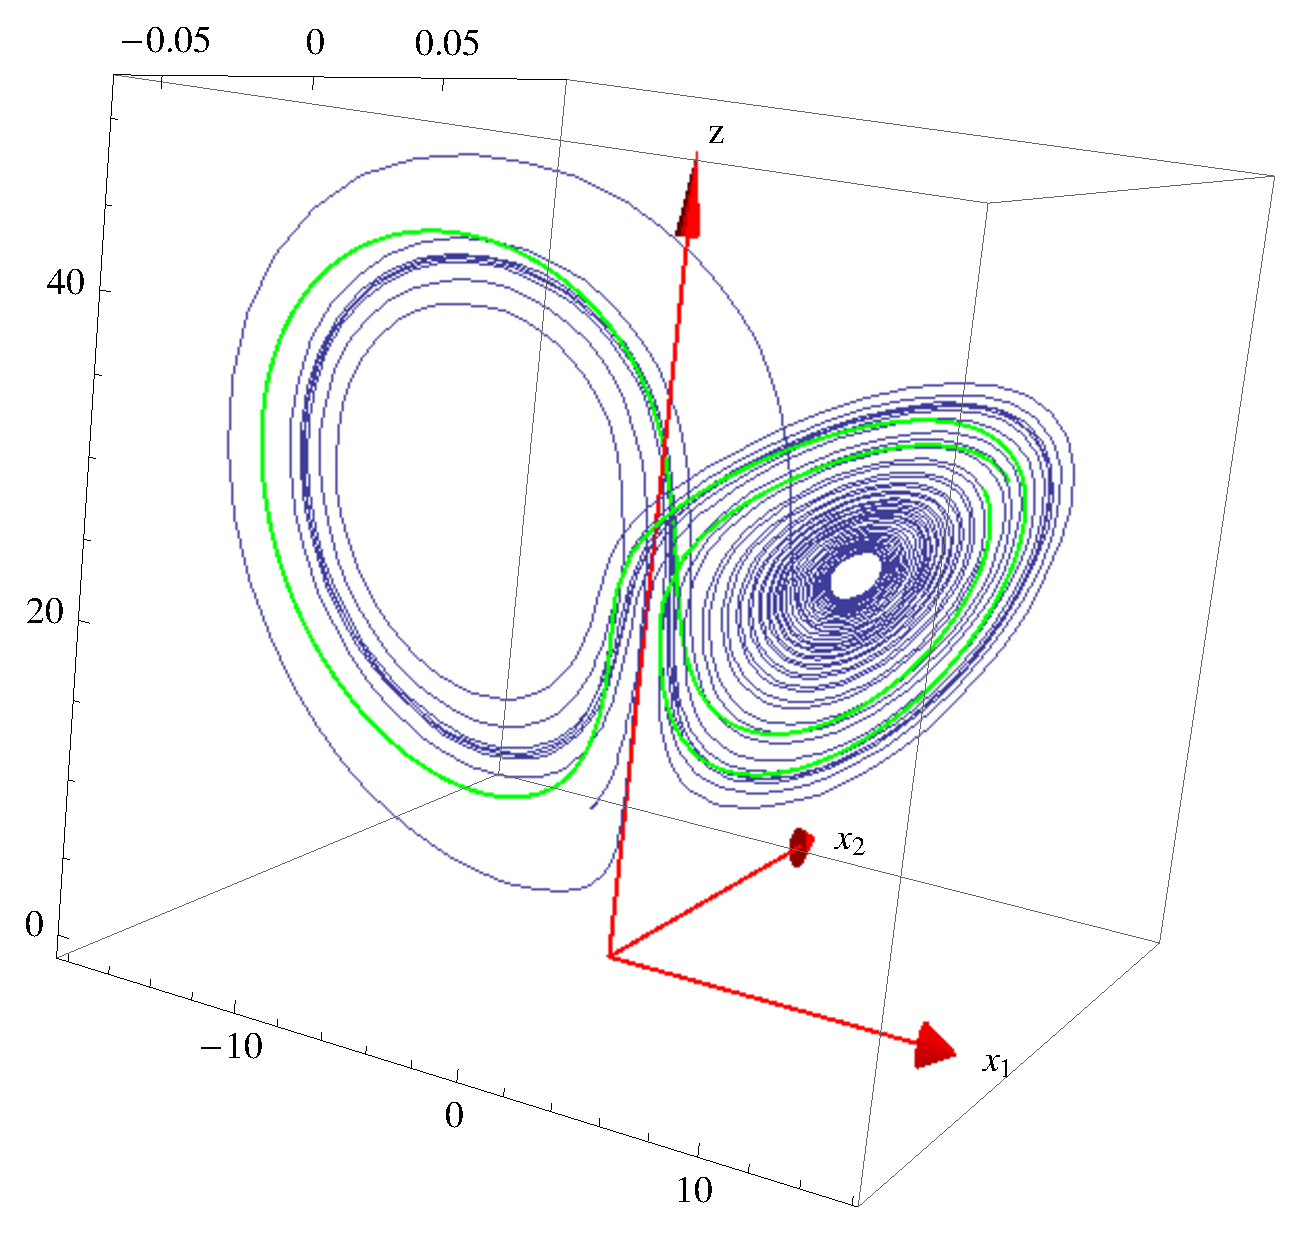
\includegraphics[width=0.45\textwidth, clip=true]{CLEtransvRPO}
(b) %\includegraphics[width=0.37\textwidth]{CLEUnrot2}
\end{center}
\caption[\CLe\ desymmetrization with transverse integration II]{
Restriction of \cLe\ dynamics on the {\slice} $\mathcal{K}$ through
\refeq{eq:difeqTransvII}. A trajectory initiated on the unstable
manifold of $\REQB{1}$ is shown in blue and \rpo\ ``011'' is shown
in green.
($e=1/10$, $\ImrCLor=0$).
(a) From Siminos Ph.D. thesis\rf{SiminosThesis}, (b) our
implementation.
    }
\label{fig:CLEtransvII}
\end{figure}
%%%%%%%%%%%%%%%%%%%%%%%%%%%%%%%%%%%%%%%%%%%%%%%%%%%%%%%%%%%%%%%%

\section{Conclusions}

Both the method of moving frames and integration on the
cross-section are still under development. We are not yet
sure whether either could be considered a success or failure.
The method of moving frames seems so far to produce a figure
without singularities, but it would require further work to
verify that singularities never occur. Integration on the
\csection\ also produces a smooth flow, resembling the
classical Lorenz attractor, and one could use the same tools
to analyze it. This method seems to work, although there is
no rigorous reason why it should.

Future work should investigate in more depth the viability of
the methods studied here. New methods (hopefully more
successful than the ones we have tested) with which to remove
the symmetry in the \cLe\ and multitude of other dynamical
systems with continuous symmetries need to be developed.
Siminos Ph.D. thesis\rf{SiminosThesis} addresses some of
these issues. In this project we have discussed, understood,
and tested the `moving frames' method as applied to \cLe\ in
the thesis. Much work still remains before these are viable
methods for higher-dimensional flows.

\section{Stability of \reqva}

\subsection{Hilbert polynomials}

The polynomials \refeq{eq:ipLaser} form a Hilbert basis for the \cLe.
\beq
\begin{split}
    u_1 &= x_1^2+x_2^2 \cont
    u_2 &= y_1^2+y_2^2 \cont
    u_3 &= x_1 y_2-x_2 y_1\cont
    u_4 &= x_1 y_1+x_2 y_2\cont
    u_5 &= z\,.
    \label{eq:ipLaser}
\end{split}
\eeq
In terms of the polar coordinates for the \cLe, these polynomials are
	\PC{shouldn't the first two be $\rho_1^2,\rho_2^2 $?}
\beq
\begin{split}
    u_1 &= \rho_1 \cont
    u_2 &= \rho_2 \cont
    u_3 &= - \rho_1 \rho_2 \sin \theta \cont
    u_4 &= \rho_1 \rho_2 \cos \theta \cont
    u_5 &= z\,.
    \label{eq:hilPolar}
\end{split}
\eeq
The \cLe\ in the Hilbert basis are:
\beq
\begin{split}
  \dot{u}_1 &=2\,\sigma\,(u_4-u_1)\,,\\
  \dot{u}_2 &=-2\left(\,u_2 - r_2\, u_3 -\,(r_1-u_5)\,u_4\right)\,,\\
  \dot{u}_3 &=-(\sigma\, +1)\,u_3+r_2\, u_1+e\, u_4\,,\\
  \dot{u}_4 &=-(\sigma\, +1)\,u_4+\,(r_1-u_5)\,u_1+\sigma\, u_2-e\,u_3\,,\\
  \dot{u}_5 &=u_4-b\, u_5\,.
\end{split}
\label{eq:CLEip}
\eeq
The relative equilibrium in polar coordinates is $\left( \rho_1 , \rho_2 , \theta , z \right) = \left(\sqrt{b \left(r_1 -d\right)},\sqrt{b d \left(r_1 -d\right)},\theta_Q, r_1 -d\right)$ where $d = 1+ \frac{e^2}{\left(\sigma +1 \right)^2}$ and $\theta_Q$ is the angle such that $\cos \theta_Q = \sqrt \frac{1}{d}$ and $\sin \theta_Q = -\sqrt \frac{d-1}{d}$.

So $\left( b \left(r_1 -d\right) , b d \left( r_1 -d \right) , b \left(r_1 -d\right) \sqrt{d-1}, b \left(r_1 -d\right), r_1 -d\right)$ is the relative equilibrium in this Hilbert basis.

\exercise{Hilbert basis singularities}{\label{exer:CLEipSyz}
% Predrag extracted from siminos/blog/CLEflotsam      Jun  5 2010
% also ChaosBook \example{Hilbert basis singularities}{\label{exam:CLEipSyz}
%
When one takes syzygies into account in rewriting a
dynamical system, singularities are introduced. For instance,
eliminate $u_2$ using the syzygy, and show that you get
the reduced set of equations,
	\PC{I removed
$  \dot{u}_2 = -2\left(\,\frac{u_3^2+u_4^2}{u_1} - \rho_2\, u_3
                -\,(\rho_1-u_5)\,u_4\right)
$
            }
\bea
  \dot{u}_1 &=& 2\,\sigma\,(u_4-u_1)
                \continue
  \dot{u}_3 &=& -(\sigma\, +1)\,u_3+\rho_2\, u_1+e\, u_4
                \continue
  \dot{u}_4 &=& -(\sigma\, +1)\,u_4+\,(\rho_1-u_5)\,u_1
                +\sigma\, {(u_3^2+u_4^2)}/{u_1}-e\,u_3
                \continue
  \dot{u}_5 &=& u_4-b\, u_5
\,,
\label{eq:CLEipSyz}
\eea
singular as $u_1\rightarrow 0$. (PC: check this - there might
be errors)
\authorES{}
    } %end \exer{Hilbert basis singularities}



The {\stabmat} in the Hilbert basis for the \cLe\ is
	\PC{This is [5$\times$5], but there are only 4 independent
            variables. How does that show up in the eigensystem of
	    {\stabmat}?}
\beq
\begin{split}
\mathbb{A}=
\left(
\begin{array}{ccccc}
-2 \sigma & 0 & 0 & 2 \sigma & 0\\
0 & -2 & 2 r_2 & 2 \left(r_1 - u_5\right) & -2 u_4\\
r_2 & 0 & -\left(\sigma +1 \right) & e & 0\\
\left(r_1 -u_5 \right) & \sigma & -e & -\left(\sigma +1 \right) & -u_1\\
0 & 0 & 0 & 1 & -b
\end{array}
\right)
\end{split}
\eeq

